% !TeX TS-program = xelatex

\documentclass{beamer}

\usepackage{tabularx}
\usepackage{xltxtra}
\usepackage{fontspec}
\usepackage{polyglossia}
\usepackage{makecell}
\usepackage{listings}

\usepackage{circuitikz}
\usepackage{tikz}
\usetikzlibrary{arrows.meta,calc,decorations.markings,math,arrows.meta,shapes,arrows,decorations.pathreplacing}
\usetikzlibrary{positioning}

\tikzset{block/.style = {draw, fill=white, rectangle,
		minimum height=3em, minimum width=2cm},
	input/.style = {coordinate},
	output/.style = {coordinate},
	pinstyle/.style = {pin edge={to-,t,black}},
	radiation/.style={decorate,decoration={expanding waves,angle=12,segment length=4pt}}
}

\setbeamertemplate{endpage}{%
	\begin{frame}
		\begin{center}
			\Huge Demo
		\end{center}
	\end{frame}
}


\setdefaultlanguage{german}

\usetheme[blue]{Verona}
\usefonttheme{default}
\usefonttheme{professionalfonts}

\usefonttheme[stillsansseriftext]{serif}

\defaultfontfeatures{Ligatures=TeX,Scale=MatchLowercase}
\setsansfont{Segoe UI Light}
\setmainfont{Segoe UI}
\setmonofont{Impact}


\title{Message Queuing Telemetry Transport}
\subtitle{Implementierung einer IoT-Anwendung auf Basis von MQTT}
\author{Maximilian Gaul, Lukas Dorner}
\date{01.07.2019}

%\mode<presentation>

\begin{document}
	
\begin{frame}
	\titlepage
\end{frame}

\begin{frame}

\frametitle{MQTT}
\framesubtitle{Control Packet}
Besteht aus bis zu drei Teilen:
\begin{itemize}
	\item \textbf{Fixed Header} - in allen MQTT Paketen vorhanden
	\item \textbf{Variable Header}
	\item \textbf{Payload}
\end{itemize}

\end{frame}

\begin{frame}

\frametitle{MQTT}
\framesubtitle{Fixed Header}
\begin{tabular}{|c|*{9}{p{9.27mm}|}}
	\hline
	\textbf{Bit $\rightarrow$} & 7 & 6 & 5 & 4 & 3 & 2 & 1 & 0\\
	\hline
	Byte 1 & \multicolumn{4}{c|}{MQTT Control Packet type} & \multicolumn{4}{p{45mm}|}{Flags specific to each MQTT Control Packet type}\\
	\hline
	Byte 2 & \multicolumn{8}{c|}{Remaining Length}\\
	\hline
\end{tabular}

\end{frame}

\begin{frame}

\frametitle{MQTT}
\framesubtitle{Fixed Header - Byte 1}
\begin{itemize}
	\item \textit{Control Packet Type}[7:4] gibt an, welche Art von Paket versendet wird:
	\begin{itemize}
		\item \begin{tabular}{ll}
			\textit{CONNECT} & Client will sich mit dem Server verbinden
		\end{tabular}
		\item \begin{tabular}{ll}
			\textit{CONNACK} & Verbindungs-\textit{ACK}
		\end{tabular}
		\item \begin{tabular}{ll}
			\textit{PUBLISH} & \hspace*{1em}\makecell[l]{Sensor schickt neuen Wert an Server}
		\end{tabular}
		\item \begin{tabular}{ll}
			\textit{SUBSCRIBE} & \makecell[l]{Client \textit{abonniert} ein Thema,\\Server leitet \textit{PUBLISH} weiter an Abonnenten}
		\end{tabular}
	\end{itemize}
	\item \textit{Flag}[3:0] sind spezifisch je nach Control Packet Type gesetzt\\
	ungültige Flags führen zu einem Schließen der Verbindung durch den Empfänger
	\begin{itemize}
		\item \begin{tabular}{ll}
			\textit{DUP} & \makecell[l]{$0$ := Erster Versuch, ein \textit{PUBLISH} zu senden,\\$1$ := Möglicherweise erneutes Senden eines \textit{PUBLISH}}
		\end{tabular}
		\item \begin{tabular}{ll}
			\textit{QoS} & \makecell[l]{Gibt an, wie oft ein \textit{PUBLISH} maximal bzw. minimal gesendet wird\\$0$ := höchstens einmal versendet}
		\end{tabular}
			\item \begin{tabular}{ll}
		\textit{RETAIN} & \makecell[l]{$1$ := Server \textit{muss} Nachricht speichern \& an \textit{zukünftige}\\\hspace*{2em}Abonnenten senden\\$0$ := Server \textit{darf nicht} $1$}
	\end{tabular}
	\end{itemize}
\end{itemize}

\end{frame}

\begin{frame}
\frametitle{MQTT}
\framesubtitle{Fixed Header - Byte 2}
\begin{itemize}
	\item Gibt die Anzahl der verbleibenden Bytes in diesem Paket an (beinhaltet den \textit{variablen} Header und die \textit{Payload}), maximal 4 Bytes lang
	\item Das \textit{höchstwertige} Bit eines Bytes gibt an, ob noch ein weiteres Byte für die Kodierung der verbleibenden Länge verwendet wurde\\
	$\Rightarrow$ Es können \textit{Control} Packets bis zu einer Größe von 256 MB kodiert werden
\end{itemize}

\end{frame}

\begin{frame}

\frametitle{MQTT}
\framesubtitle{Variable Header}
\begin{itemize}
	\item Unterschiedliche Bedeutung je nach \textit{Control Packet Type}
	\begin{itemize}
		\item Zuordnung von \textit{PUBLISH} Paketen mit \textit{QoS} $> 0$ z.B. über einen 16 Bit Identifier
		\item \textit{PUBLISH} mit \textit{QoS} = $0$ darf keinen Packet Identifier enthalten
		\item Bei einem \textit{CONNECT} Paket definiert er wichtige Verbindungseigenschaften
	\end{itemize}
\end{itemize}

\end{frame}

\begin{frame}

\frametitle{MQTT}
\framesubtitle{Payload}
\begin{itemize}
	\item \textit{CONNECT}, \textit{SUBSCRIBE} und \textit{UNSUBSCRIBE} haben immer eine Payload
	\item \textit{PUBLISH} Pakete auch ohne Payload
\end{itemize}

\end{frame}

\begin{frame}

\frametitle{MQTT}
\framesubtitle{Verbindungsaufbau}
\begin{itemize}
	\item 
\end{itemize}

\end{frame}

\begin{frame}

\frametitle{MQTT}
\framesubtitle{Verbindungsabbau}
\begin{itemize}
	\item 
\end{itemize}

\end{frame}

\begin{frame}

\frametitle{MQTT}
\framesubtitle{Netzwerk \& Sicherheit}
\begin{itemize}
	\item Als Transportprotokoll kann z.B. \textit{TCP}, \textit{TLS} oder \textit{WebSocket} verwendet werden
	\begin{itemize}
		\item \textit{UDP} ist ungeeignet, da \textit{verbindungslos} - keine Garantie für Zustellung der Daten
	\end{itemize}
	\item \textit{MQTT} sieht sich selbst nur als Transportprotokoll, für Sicherheit zu sorgen liegt in der Verantwortung des Implementierenden
	\begin{itemize}
		\item Empfiehlt \textit{TLS}
	\end{itemize}
\end{itemize}

\end{frame}

\begin{frame}

\frametitle{Projekt}
\framesubtitle{Grundlegender Aufbau}
\begin{tikzpicture}
	\node (A) [anchor=south west,inner sep=0] at (0,0) {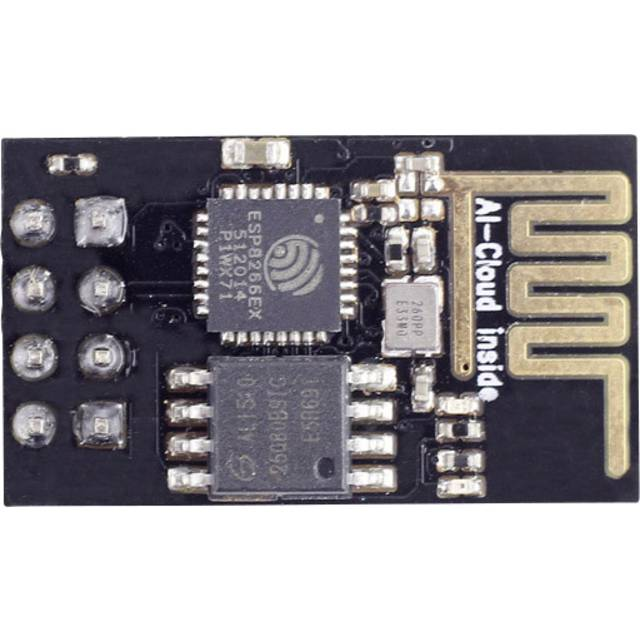
\includegraphics[scale=0.1]{images/esp8266.jpg}};
	\node (B) [right = of A] at (0,0) {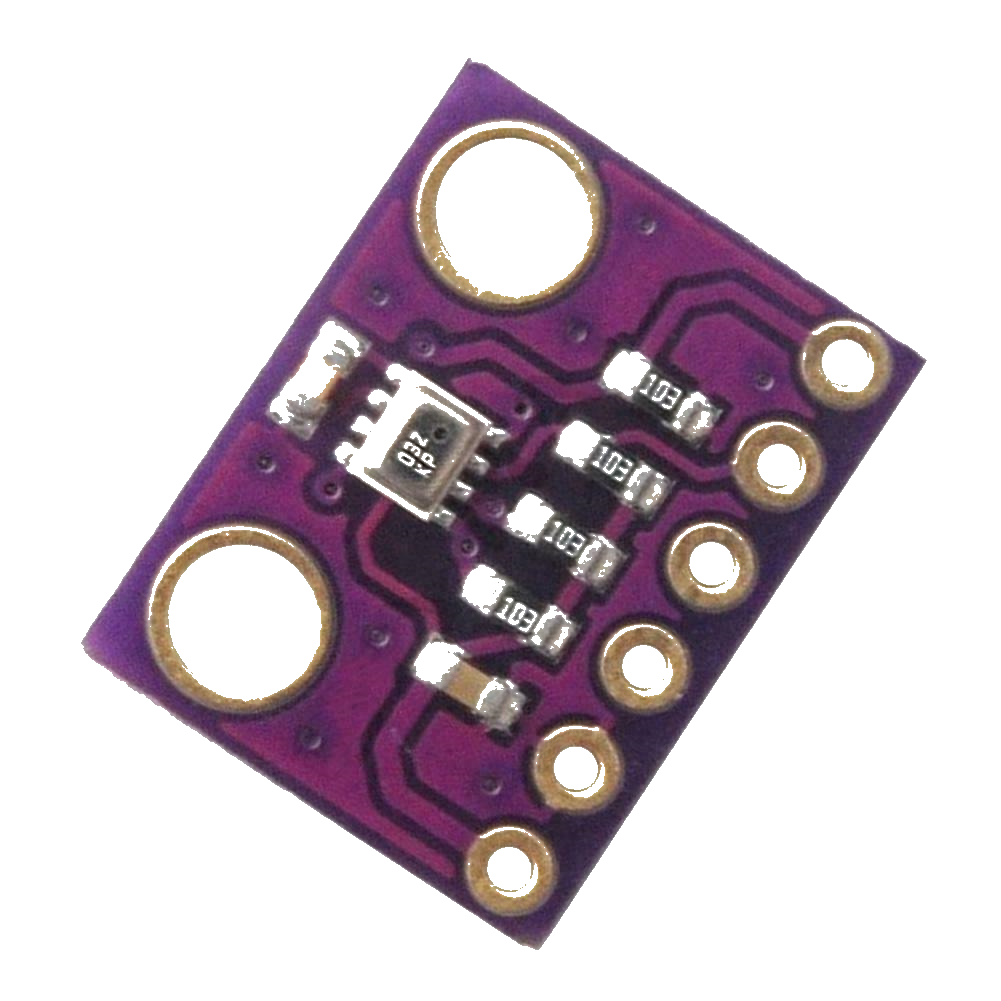
\includegraphics[scale=0.037]{images/bmp280.png}};
	\node (C) [below = of B] {ESP8266 + BMP280};
	
	\node (D) [right = 8cm of B] at (0,0) {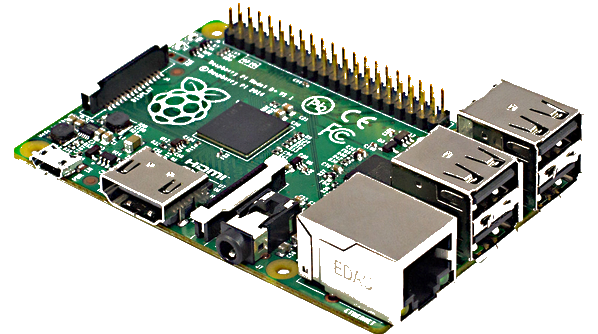
\includegraphics[scale=0.175]{images/raspi.png}};
	\node (E) [below = of D] {Raspberry Pi + Mosquitto};
	
	\draw[radiation] ([shift={(1cm,2cm)}]A)-- node [above=7mm] {MQTT PUBLISH} ([shift={(-1cm,2cm)}]D);
\end{tikzpicture}

\end{frame}

\begin{frame}

\frametitle{Projekt}
\framesubtitle{BMP280}
\begin{tabularx}{\textwidth}{Xr}
	\begin{itemize}
		\item Anbindung über den $I^2C$-Bus (\textit{Inter Integrated Circuit})
		\item Temperatur- und Drucksensor mit einer Auflösung von bis zu 20 Bit
		\item Ausgelesene Werte verrechnet mit voreingestellten\\Kalibrationsparametern ergeben Temperatur
	\end{itemize} & \raisebox{-1\height}{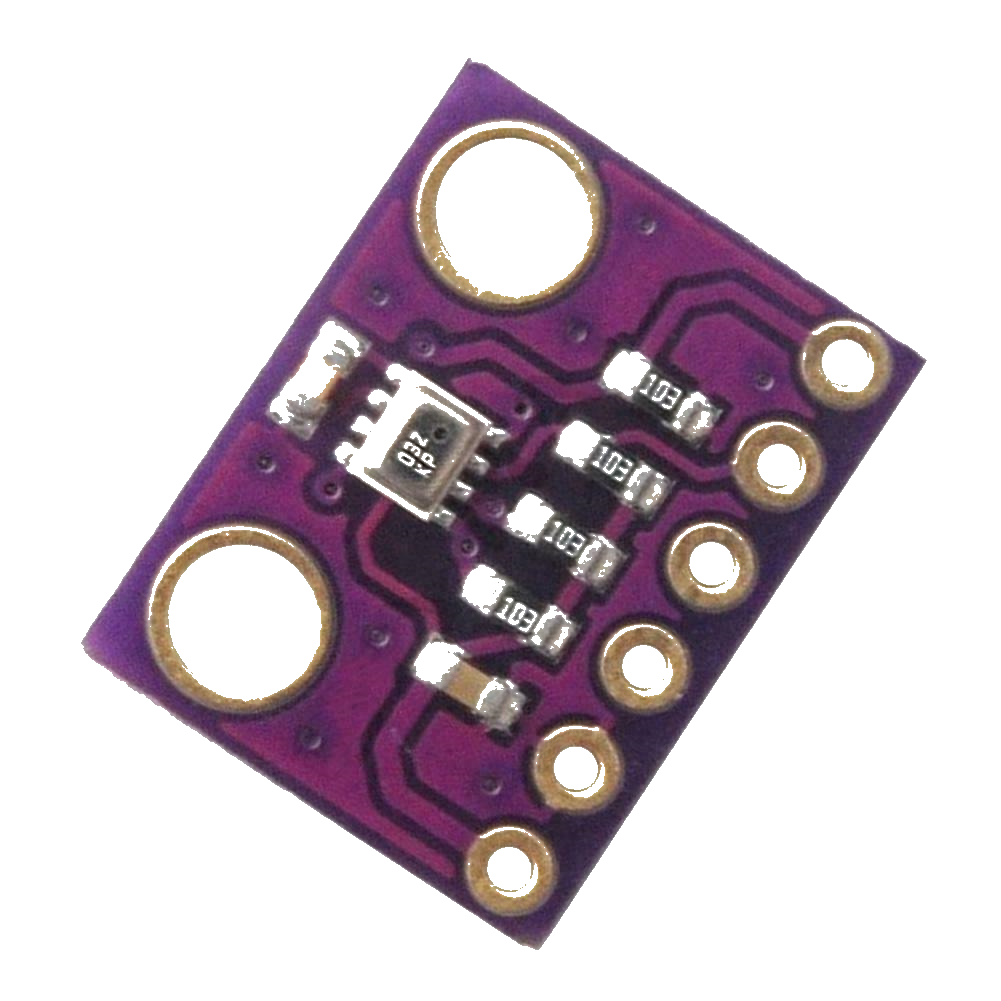
\includegraphics[scale=0.075]{images/bmp280.png}}
\end{tabularx}

\end{frame}

\begin{frame}

\frametitle{Projekt}
\framesubtitle{ESP8266}
\begin{tabularx}{\textwidth}{rX}
	\raisebox{-1.33\height}{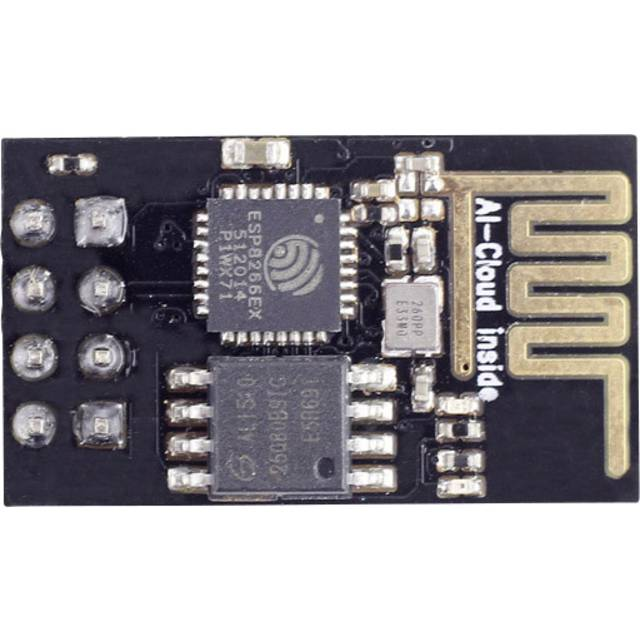
\includegraphics[scale=0.175]{images/esp8266.jpg}} & \begin{itemize}
		\item Unterstützt 802.11 b/g/n mit bis zu 72.2Mbps
		\item Antenne als Leiterbahn auf der Platine
		\item Tensilica L106 32-bit \textit{RISC} mit bis zu 160 MHz (mit \textit{PLL-OC} auch > 300 MHz)
		\item 96 KByte RAM
		\item 4 MB Flash Speicher, per \textit{SPI} angebunden
		\item Ursprünglich als \textit{dummer}, nur per \textit{AT}-Kommandos bedienbarer WiFi-Chip verkauft
		\item Nach viel \textit{Reverse-Engineering} der Community und schließlich Freigeben eines \textit{SDK} durch den Hersteller heute frei programmierbar (z.B. mit \textit{Arduino} oder in \textit{C} / \textit{Assembler})
	\end{itemize}
\end{tabularx}

\end{frame}

\begin{frame}

\frametitle{Projekt}
\framesubtitle{ESP8266 Firmware}
\begin{itemize}
	\item Implementierung der \textit{Master}-$I^2C$-Schnittstelle in Software (kein \textit{HW-I2C})
	\item Implementierung des \textit{MQTT-PUBLISH}-Paketes
	\item 10s Software-Timer:
	\begin{itemize}
		\item Temperatur messen
		\item MQTT-PUBLISH Paket erstellen
		\item Mit Raspi per TCP verbinden und Paket über WiFi verschicken
	\end{itemize}
\end{itemize}

\end{frame}

\begin{frame}

\frametitle{Projekt}
\framesubtitle{Raspberry Pi}
\begin{itemize}
	\item 
\end{itemize}

\end{frame}


\usebeamertemplate{endpage}


\end{document}